\documentclass[a4paper,11.5pt]{article}
\usepackage[textwidth=170mm, textheight=230mm, inner=20mm, top=20mm, bottom=30mm]{geometry}
\usepackage[normalem]{ulem}
\usepackage[utf8]{inputenc}
\usepackage[T1]{fontenc}
\PassOptionsToPackage{defaults=hu-min}{magyar.ldf}
\usepackage[magyar]{babel}
\usepackage{amsmath, xcolor, amsthm,amssymb,paralist,array, ellipsis, graphicx, tikz}
\usetikzlibrary{shapes.geometric, arrows, positioning}
%\usepackage{marvosym}

\usepackage{listings}
\lstset{
	language=C++, 
	basicstyle=\ttfamily, 
	keywordstyle=\color{blue}\ttfamily, 
	stringstyle=\color{red}\ttfamily,
	tabsize = 4
}

\makeatletter
\renewcommand*{\mathellipsis}{%
	\mathinner{%
		\kern\ellipsisbeforegap%
		{\ldotp}\kern\ellipsisgap%
		{\ldotp}\kern\ellipsisgap%
		{\ldotp}\kern\ellipsisaftergap%
	}%
}
\renewcommand*{\dotsb@}{%
	\mathinner{%
		\kern\ellipsisbeforegap%
		{\cdotp}\kern\ellipsisgap%
		{\cdotp}\kern\ellipsisgap%
		{\cdotp}\kern\ellipsisaftergap%
	}%
}
\renewcommand*{\@cdots}{%
	\mathinner{%
		\kern\ellipsisbeforegap%
		{\cdotp}\kern\ellipsisgap%
		{\cdotp}\kern\ellipsisgap%
		{\cdotp}\kern\ellipsisaftergap%
	}%
}
\renewcommand*{\ellipsis@default}{%
	\ellipsis@before
	\kern\ellipsisbeforegap
	.\kern\ellipsisgap
	.\kern\ellipsisgap
	.\kern\ellipsisgap
	\ellipsis@after\relax}
\renewcommand*{\ellipsis@centered}{%
	\ellipsis@before
	\kern\ellipsisbeforegap
	.\kern\ellipsisgap
	.\kern\ellipsisgap
	.\kern\ellipsisaftergap
	\ellipsis@after\relax}
\AtBeginDocument{%
	\DeclareRobustCommand*{\dots}{%
		\ifmmode\@xp\mdots@\else\@xp\textellipsis\fi}}
\def\ellipsisgap{.1em}
\def\ellipsisbeforegap{.05em}
\def\ellipsisaftergap{.05em}
\makeatother

\usepackage{hyperref}

\begin{document}
	%%%%%%%%%%%RÖVIDÍTÉSEK%%%%%%%%%%
	\setlength\parindent{0pt}
	\def\s{\hspace{0.2mm}\vphantom{\beta}}
	\def\Z{\mathbb{Z}}
	\def\Q{\mathbb{Q}}
	\def\R{\mathbb{R}}
	\def\C{\mathbb{C}}
	\def\N{\mathbb{N}}
	\def\Ra{\overline{\mathbb{R}}}
	
	\def\sume{\displaystyle\sum_{n=1}^{+\infty}}
	\def\sumn{\displaystyle\sum_{n=0}^{+\infty}}
	
	\def\narrow{\underset{n\rightarrow+\infty}{\longrightarrow}}
	\def\limn{\displaystyle\lim_{n\to +\infty}}
	\def\limx{\displaystyle\lim_{x\to +\infty}}
	
	\theoremstyle{definition}
	\newtheorem{theorem}{Tétel}[subsection] 
	
	\theoremstyle{definition}
	\newtheorem{definition}[theorem]{Definíció} 
	\newtheorem{example}[theorem]{Példa} 
	\newtheorem{task}[theorem]{Feladat} 
	\newtheorem{note}[theorem]{Megjegyzés}
	%%%%%%%%%%%%%%%%%%%%%%%%%%%%%%%%%%%%%%%%%%%%%%%%%%%%%%%%%%%%%%%%%%%%%
	\begin{center}
		{\LARGE\textbf{C++}}
		
		{\Large Gyakorlat jegyzet}
		
		2 óra.
	\end{center}
	A jegyzetet \textsc{Umann} Kristóf készítette \textsc{Porkoláb} Zoltán és \textsc{Horváth} Gábor. (\today)
	
	%TODO függvény és operátor túlterhelés ide illene a legjobban
	%TODO globális és statikus függvényeket is ide kéne beilleszteni
	
	
	\section{Láthatóság, élettartam}
	Egy objektum \textbf{láthatóságának} nevezzük a kódnak azon szakaszait, melyeknél lehet rá hivatkozni.
	\smallskip
	
	Egy objektum \textbf{élettartamának} nevezzük a kód azon szakaszát, melynél bent szerepel a memóriában. Amikor egy objektum élettartama elkezdődik, azt mondjuk, az objektum létrejön, míg az élettartam végén az objektum megsemmisül.
	\medskip
	\begin{note}
		Ez alapján megállapíthatjuk, hogy egy globális változó láthatósága és élettartama a program futásának elejétől végéig tart.
	\end{note}
	
	Figyeljük meg, mikor tudunk \texttt{x} változóra hivatkozni (azaz hol lesz \texttt{x} látható)!
	\begin{lstlisting}
int x;

int main()
{
	int x = 1;
	{
		int x = 2;
		std::cout << x << std::endl; // 2
	}
}
	\end{lstlisting}
	Megfigyelhető, hogy a \texttt{main} függvény elején létrehozott \texttt{x} az utána következő blokkban teljesen elérhetetlen -- nincs olyan szabványos nyelvi eszköz, amivel tudnánk rá hivatkozni. Ezt a folyamatot \textbf{leárnyékolás}nak (\textit{shadowing}) nevezzük. Azonban a külső, globális \texttt{x}-re bármikor tudunk hivatkozni az alábbi módon:
	\begin{lstlisting}
int x;

int main()
{
	int x = 1;
	{
		int x = 2;
		std::cout << ::x << std::endl; // 0
	}
}
	\end{lstlisting}
	
	\section{A stack működése}
	A stack a c++ alapértelmezett ,,memóriája'', minden változó alapértelmezetten itt jön létre és semmisül meg. Amennyiben egy változóra többet nem tudunk hivatkozni, automatikusan megsemmisül.
	
	\begin{lstlisting}
#include <iostream>

int f()
{
	int x = 0; //x letrejon
	++x;
	return x;
} //x megsemmisul

int main()
{
	for (int i = 0; i<5; i++)
		std::cout << f() << ' '; // 1 1 1 1 1
}
	\end{lstlisting}
	\medskip
	
	A fenti kód működését így képzelhetjük el:
	
	%durva kód copy paste inc... dont be mad :'(
	\begin{center}
		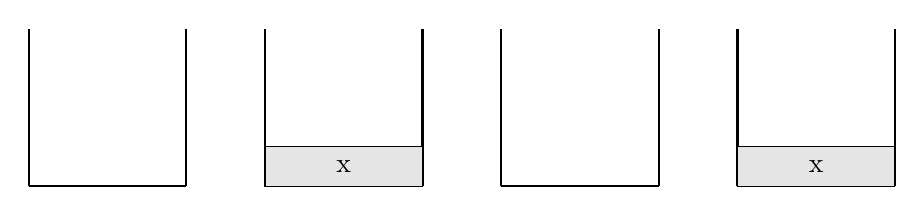
\begin{tikzpicture}
		\tikzstyle{Node} = [rectangle, minimum width=2cm, minimum height=5mm, text centered, draw=black, fill= gray!20]
		\tikzstyle{arrow} = [thick,->,>=stealth]
		
		
		\draw [thick, black] (-3, 0) -- (-1, 0);
		\draw [thick, black] (-3, 0) -- (-3, 2);
		\draw [thick, black] (-1, 0) -- (-1, 2);
		
		\draw [thick, black] (0, 0) -- (2, 0);
		\draw [thick, black] (0, 0) -- (0, 2);
		\draw [thick, black] (2, 0) -- (2, 2);
		\node (x) [Node] at (1,0.25) {x};
		
		\draw [thick, black] (3, 0) -- (5, 0);
		\draw [thick, black] (3, 0) -- (3, 2);
		\draw [thick, black] (5, 0) -- (5, 2);
		
		\draw [thick, black] (6, 0) -- (8, 0);
		\draw [thick, black] (6, 0) -- (6, 2);
		\draw [thick, black] (8, 0) -- (8, 2);
		\node (x) [Node] at (7,0.25) {x};
		\end{tikzpicture}
	\end{center}
	Az ábrán egy stack-et látunk. Amikor a vezérlés az \texttt{f} függvényhez ér, és ott létrehozza az \texttt{x} változót, azt behelyezi a stack-be. A \texttt{return} kulcsszó hatására készít \texttt{x}-ről egy temporális példányt, ami a függvény visszatérési értéke lesz. Amikor a vezérlés visszatér a \texttt{main} függvényhez, {x}-re nem tudunk tovább hivatkozni, így azt megsemmisíti, és ez ismétlődik folyamatosan.
	\smallskip
	
	A stack egy FILO (\textit{first in last out}) adatszerkezet -- azaz azt az elemet ,,dobja'' ki a vezérlés a stack-ből, melyet utoljára rakott be.
	
	\section{Paraméter átvétel}
	\subsection{Érték szerinti paraméter átvétel}
	Próbáljuk megvalósítani a swap függvényt!
	%http://tex.stackexchange.com/questions/228724/how-do-i-make-tikz-make-a-curved-arrow-from-one-node-to-another-when-my-nodes-ar
	\begin{lstlisting}
#include <iostream>
void swapWrong(int a, int b)
{
	int tmp = a;
	a = b;
	b = a;
}

int main()
{
	int c = 5, d = 8;
	swap(c, d);
	std::cout << c << ' ' << d << std::endl;
}
	\end{lstlisting}		
	A program kimenete \texttt{5 8} ment. Ez egy teljesen jól definiált viselkedés. Ez azért van, mert itt \textbf{érték} szerint vettük át (\textit{pass by value}) \texttt{a} és \texttt{b} változót. A következő ábrán megfigyelhetjük miért is nem. Képzeljük el, ahogy ebbe a verembe a kódunk elrakja a \texttt{c} és \texttt{d} változókat. Majd meghívja a \texttt{swapWrong} függvényt, melyben létrehozott \texttt{a} és \texttt{b} változókat ismét behelyezi. Bár a függvényre lokális \texttt{a} és \texttt{b} változókat megcseréli, de a függvényhívás után ezeket ki is törli a stackből.
	\begin{center}
		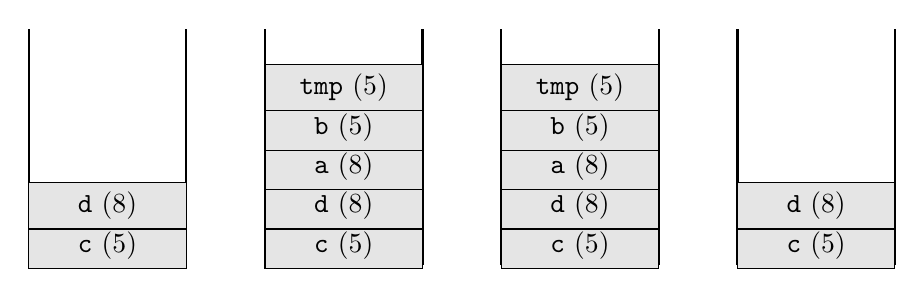
\begin{tikzpicture}
		\tikzstyle{Node} = [rectangle, minimum width=2cm, minimum height=5mm, text centered, draw=black, fill= gray!20]
		\tikzstyle{arrow} = [thick,->,>=stealth]
		
		\draw [thick, black] (0, 0) -- (2, 0);
		\draw [thick, black] (0, 0) -- (0, 3);
		\draw [thick, black] (2, 0) -- (2, 3);
		\node (c2) [Node] at (1,0.25) {\texttt{c} (5)};
		\node (d2) [Node] at (1,0.75) {\texttt{d} (8)};
		
		\draw [thick, black] (3, 0) -- (5, 0);
		\draw [thick, black] (3, 0) -- (3, 3);
		\draw [thick, black] (5, 0) -- (5, 3);
		\node (c3) [Node] at (4,0.25) {\texttt{c} (5)};
		\node (d3) [Node] at (4,0.75) {\texttt{d} (8)};
		\node (a3) [Node] at (4,1.25) {\texttt{a} (8)};
		\node (b3) [Node] at (4,1.75) {\texttt{b} (5)};
		\node (b3) [Node] at (4,2.25) {\texttt{tmp} (5)};
		
		\draw [thick, black] (6, 0) -- (8, 0);
		\draw [thick, black] (6, 0) -- (6, 3);
		\draw [thick, black] (8, 0) -- (8, 3);
		\node (c3) [Node] at (7,0.25) {\texttt{c} (5)};
		\node (d3) [Node] at (7,0.75) {\texttt{d} (8)};
		\node (a3) [Node] at (7,1.25) {\texttt{a} (8)};
		\node (b3) [Node] at (7,1.75) {\texttt{b} (5)};
		\node (b3) [Node] at (7,2.25) {\texttt{tmp} (5)};
		
		\draw [thick, black] (9, 0) -- (11, 0);
		\draw [thick, black] (9, 0) -- (9, 3);
		\draw [thick, black] (11, 0) -- (11, 3);
		\node (a4) [Node] at (10,0.25) {\texttt{c} (5)};
		\node (b4) [Node] at (10,0.75) {\texttt{d} (8)};
		\end{tikzpicture}
		\smallskip
		
		Tekintsünk el a \texttt{tmp} változótól.
	\end{center}
	C++ban alapértelmezett a paraméterátadás függvényeknél érték szerint történik.
	\subsection{Mutatóval történő paraméter átvétel}
	A mutatók olyan nyelvi elemek, melyek egy memóriaterületre mutatnak. Segítségükkel anélkül is tudunk hivatkozni egy adott objektumra (és nem csak a másolatára), hogy közvetlenül az objektummal dolgoznánk. Most röviden megismerkedünk velük, de később részletesebben visszatérünk rájuk.
	\begin{lstlisting}
int main()
{
	int c = 5, d = 8;
	int *p = &c;
}
	\end{lstlisting}
	A fenti példában \texttt{p} egy mutató (\textit{pointer}), mely egy \texttt{int} típusra mutat. Ahhoz, hogy értéket tudjunk adni egy mutatónak, egy memóriacímet (\textit{referenciát}) kell neki értékül adni, amire rá tud mutatni, erre való a \textbf{referáló operátor} (\&). Ha a mutató által \textit{mutatott értéket} szeretnénk módosítani, akkor dereferálnunk kell a \textbf{dereferáló operátor}ral (*).
	\begin{lstlisting}
int *p = &c; //referaljuk c-t
*p = 4; //dereferaljuk p-t
p = &d;
*p = 7;
	\end{lstlisting}
	Rendre: pointer inicializálása, pointer által mutatott érték módosítása, pointer átállítása másik memóriacímre, és a mutatott érték módosítása.
	
	Egy mutató mutathat változóra, másik mutatóra, saját magára, és sehova is. Azok a mutatókak, melyek sehová sem mutatnak, nullpointernek nevezzük, és így hozhatjuk létre őket:
	
	{\centering \texttt{p = 0;\quad \quad p = NULL;\quad \quad p = nullptr;} \par}
	
	\begin{note}
		Ez a három értékadás (közel) ekvivalens, azonban a \texttt{nullptr} kulcsszó csak c++11ben érhető el.
	\end{note}
	
	\begin{lstlisting}
void swapP(int *a, int *b)
{
	int tmp = *a;
	*a = *b;
	*b = tmp;
}
	\end{lstlisting}
	
	Amennyiben ezt a függvényt hívjuk meg, valóban megcserélődik a két változó értéke. De ehhez fontos, hogy ne simán \texttt{swapP(c, d)}-t írjunk függvényhívásként, az ugyanis az fordítási hibához vezetne, mert a \texttt{c} és \texttt{d} típusa \texttt{int}, és nem \texttt{int*}. Ahhoz, hogy értéket adjunk egy pointernek, a \texttt{c}-hez és \texttt{d}-hez tartozó memóriacímeket kell átadni, így a \texttt{swapP(\&c, \&d)} hívás lesz megfelelő.
	\begin{center}
		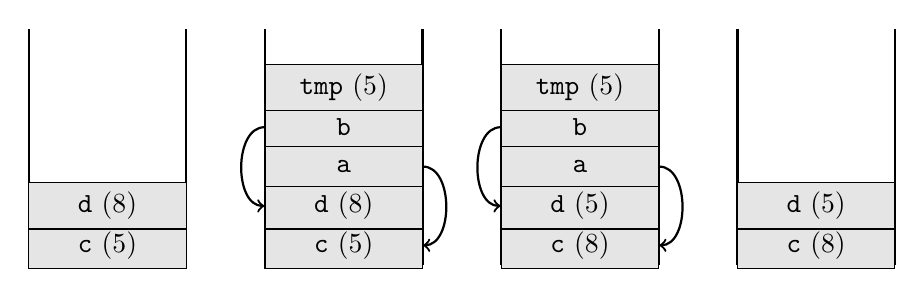
\begin{tikzpicture}
		\tikzstyle{Node} = [rectangle, minimum width=2cm, minimum height=5mm, text centered, draw=black, fill= gray!20]
		\tikzstyle{arrow} = [thick,->,>=stealth]
		
		\draw [thick, black] (-3, 0) -- (-1, 0);
		\draw [thick, black] (-3, 0) -- (-3, 3);
		\draw [thick, black] (-1, 0) -- (-1, 3);
		\node (c1) [Node] at (-2,0.25) {\texttt{c} (5)};
		\node (d1) [Node] at (-2,0.75) {\texttt{d} (8)};
		
		\draw [thick, black] (0, 0) -- (2, 0);
		\draw [thick, black] (0, 0) -- (0, 3);
		\draw [thick, black] (2, 0) -- (2, 3);
		\node (c2) [Node] at (1,0.25) {\texttt{c} (5)};
		\node (d2) [Node] at (1,0.75) {\texttt{d} (8)};
		\node (a2) [Node] at (1,1.25) {\texttt{a}};
		\node (b2) [Node] at (1,1.75) {\texttt{b}};
		\node (tmp2) [Node] at (1,2.25) {\texttt{tmp} (5)};
		
		\path[every node/.style={font=\sffamily\small}]
			(a2) edge[bend left = 90, thick, ->] node [right] {} (c2);
		\path[every node/.style={font=\sffamily\small}]
			(b2) edge[bend right = 90, thick, ->] node [left] {} (d2);
		
		\draw [thick, black] (3, 0) -- (5, 0);
		\draw [thick, black] (3, 0) -- (3, 3);
		\draw [thick, black] (5, 0) -- (5, 3);
		\node (c3) [Node] at (4,0.25) {\texttt{c} (8)};
		\node (d3) [Node] at (4,0.75) {\texttt{d} (5)};
		\node (a3) [Node] at (4,1.25) {\texttt{a}};
		\node (b3) [Node] at (4,1.75) {\texttt{b}};
		\node (tmp3) [Node] at (4,2.25) {\texttt{tmp} (5)};
		
		
		\path[every node/.style={font=\sffamily\small}]
		(a3) edge[bend left = 90, thick, ->] node [right] {} (c3);
		\path[every node/.style={font=\sffamily\small}]
		(b3) edge[bend right = 90, thick, ->] node [left] {} (d3);
		
		\draw [thick, black] (6, 0) -- (8, 0);
		\draw [thick, black] (6, 0) -- (6, 3);
		\draw [thick, black] (8, 0) -- (8, 3);
		\node (a4) [Node] at (7,0.25) {\texttt{c} (8)};
		\node (b4) [Node] at (7,0.75) {\texttt{d} (5)};
		\end{tikzpicture}
	\end{center}
	
	Ezt azonban ez még mindig \textbf{érték szerinti} átadásnak nevezzük, mert most nem konkrét értéket, hanem a memóriacímet másoltuk át.
	
	\begin{lstlisting}
void swapWrong2(int *a, int *b)
{
	int *tmp = a;
	a = b;
	b = tmp;
}
	\end{lstlisting}
	Ebben a példában nem a pointerek által mutatott értéket, hanem magukat a pointereket cseréljük meg. Itt annyi fog csupán történni, hogy a függvény beljesében \texttt{a} és \texttt{b} pointer másra fog mutatni. De annak értéke nem változik.
	
	\begin{center}
		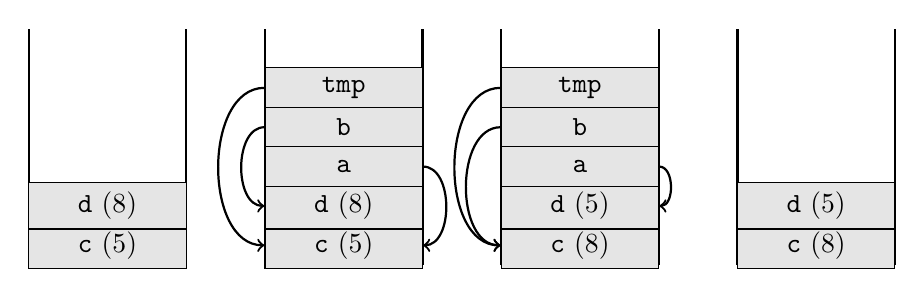
\begin{tikzpicture}
		\tikzstyle{Node} = [rectangle, minimum width=2cm, minimum height=5mm, text centered, draw=black, fill= gray!20]
		\tikzstyle{arrow} = [thick,->,>=stealth]
		
		\draw [thick, black] (-3, 0) -- (-1, 0);
		\draw [thick, black] (-3, 0) -- (-3, 3);
		\draw [thick, black] (-1, 0) -- (-1, 3);
		\node (c1) [Node] at (-2,0.25) {\texttt{c} (5)};
		\node (d1) [Node] at (-2,0.75) {\texttt{d} (8)};
		
		\draw [thick, black] (0, 0) -- (2, 0);
		\draw [thick, black] (0, 0) -- (0, 3);
		\draw [thick, black] (2, 0) -- (2, 3);
		\node (c2) [Node] at (1,0.25) {\texttt{c} (5)};
		\node (d2) [Node] at (1,0.75) {\texttt{d} (8)};
		\node (a2) [Node] at (1,1.25) {\texttt{a}};
		\node (b2) [Node] at (1,1.75) {\texttt{b}};
		\node (tmp2) [Node] at (1,2.25) {\texttt{tmp}};
		
		\path[every node/.style={font=\sffamily\small}]
		(a2) edge[bend left = 90, thick, ->] node [right] {} (c2);
		\path[every node/.style={font=\sffamily\small}]
		(b2) edge[bend right = 90, thick, ->] node [left] {} (d2);
		\path[every node/.style={font=\sffamily\small}]
		(tmp2) edge[bend right = 90, thick, ->] node [left] {} (c2);
		
		\draw [thick, black] (3, 0) -- (5, 0);
		\draw [thick, black] (3, 0) -- (3, 3);
		\draw [thick, black] (5, 0) -- (5, 3);
		\node (c3) [Node] at (4,0.25) {\texttt{c} (8)};
		\node (d3) [Node] at (4,0.75) {\texttt{d} (5)};
		\node (a3) [Node] at (4,1.25) {\texttt{a}};
		\node (b3) [Node] at (4,1.75) {\texttt{b}};
		\node (tmp3) [Node] at (4,2.25) {\texttt{tmp}};
		
		
		\path[every node/.style={font=\sffamily\small}]
		(a3) edge[bend left = 90, thick, ->] node [right] {} (d3);
		\path[every node/.style={font=\sffamily\small}]
		(b3) edge[bend right = 90, thick, ->] node [left] {} (c3);
		\path[every node/.style={font=\sffamily\small}]
		(tmp3) edge[bend right = 90, thick, ->] node [left] {} (c3);
		
		\draw [thick, black] (6, 0) -- (8, 0);
		\draw [thick, black] (6, 0) -- (6, 3);
		\draw [thick, black] (8, 0) -- (8, 3);
		\node (a4) [Node] at (7,0.25) {\texttt{c} (8)};
		\node (b4) [Node] at (7,0.75) {\texttt{d} (5)};
		\end{tikzpicture}
	\end{center}
	\subsection{Referencia szerinti paraméter átvétel}
	Megállapíthatjuk, hogy az előző megoldásnál nem változtattuk meg azt, hogy mire mutassanak a pointerek, így azokat konstansként is definiálhatnánk. A konstans pointerek módosíthatják a mutatott cím értékét, de máshova nem mutathatnak. Úgy tudunk egy ilyen pointert létrehozni, hogy a csillag után írjuk a \texttt{const} kulcsszót.
	\begin{lstlisting}
void swap(int * const a, int * const b)
{
	//...
}
	\end{lstlisting}
	Egy kis szintaktikai cukorkával megúszhatjuk azt, hogy folyton kiírjuk a \texttt{* const}-ot (lévén ritkán akarjuk megváltoztatni hogy ilyen esetben a pointer hova mutasson). Erre való a {referencia szerinti paraméter átváétel} (\textit{pass by reference}). A referencia úgy működik, mintha egy konstans pointer lenne.
	\begin{lstlisting}
void swapRef(int &a, int &b)
{
	int tmp = a;
	a = b;
	b = tmp;
}
	\end{lstlisting} 
	Ez a két függvény lényegében ekvivalensek. A különbség a referencia és a pointer között csupán annyi, hogy egy referencia nem lehet null.
	\begin{note}
		Ez bár ezt referencia szerinti átvételnek nevezzük, de itt is történik másolás, a memóriacímet ítt is érték szerint vesszük át.
	\end{note}
		Megjegyzendő, hogy a fenti \texttt{swapRef} függvénynek nem kell memóriacímeket átadni, \texttt{swapRef(a,b)}-t kell írnunk.
	\begin{note}
		Egy referenciát mindig inicializálni kell. Csak úgy mint egy konstanst (különben fordítási hibát kapunk.)
	\end{note}
	\subsection{Visszatérési érték problémája}
	Nem primitív (pl. \texttt{int}) típusoknál gyakran megeshet, hogy egy adott ípushoz tartozó pointer mérete kisebb, mint magának az objektumé, így megérheti mindentől függetlenül a paramétert referencia szerint átvenni. Ezen felbátorodva mondhatnánk azt is, hogy referenciával is térjünk vissza (a követekező példában tekintsünk el attól, hogy \texttt{int}-el dolgozunk, bátran képzeljük azt hogy az pl. egy nagyon nagy mátrix)!
	\begin{lstlisting}
int& addOne(int &i)
{
	i++;
	return i;
}

int main()
{
	int i = 0;
	int a = addOne(i);
	std::cout << a << std::endl;
}
	\end{lstlisting}
	A fenti kóddal semmi gond nincs is. De mi van, ha egy picit módosítunk rajta?
	\begin{lstlisting}
int& addOne(int &i)
{
	int ret = ++i;
	return ret;
}
	\end{lstlisting}
	A baj máris megvan, amit egy warning is jelezni fog nekünk: olyan objektumra hivatkozó referenciát adunk vissza, amely \texttt{addOne}-on belül lokális. Ez azt jelenti, hogy amint a vezérlés visszatér a \texttt{main} függvényhez, \texttt{ret} megsemmisül, és a \texttt{main} függvény pedig a \texttt{ret}-hez tartozó címen lévő értéket próbálná meg lemásolni. Mivel viszont a \texttt{ret} már ezen a ponton megsemmisült, semmi nem garantálja, hogy azon a memóriaterületen ne követekezett volna be módosítás.
	
	\medskip
	Az olyan memóriaterületre való hivatkozás, mely nincs a program számára lefoglalva, nem definiált viselkedést eredményez.
	\begin{note}
		Értelemszerűen pointerekkel ez ugyanúgy probléma.
	\end{note}
	\section{Statikus változók/függvények}
	Statikus változó többféle van -- függően attól, hogy a definíciójukhoz szükséges \texttt{static} kulcsszót milyen kontextusba írjuk, egy másfajta változót kapunk. Működésük sokban hasonlít a globálisokéhoz.
	\subsection{Fordítási egységre statikus változók}
	A függvényen és névteren kívül deklarált statikus változók az adott fordítási egységre lokálisak -- élettartamuk a futás elejétől végigtartamig tart, és kizárólagosan az adott fordítási egységben láthatóak.
	\medskip
	
	\fbox{\textbf{main.cpp}}
	\begin{lstlisting}
#include <iostream>

static int x;

int main()
{
	x = 2;
}
	\end{lstlisting}
	\medskip
	
	\fbox{\textbf{other.cpp}}
	\begin{lstlisting}
#include <iostream>

static int x;

void f()
{
	x = 0;
}
	\end{lstlisting}
	Ha ezt a két fájlt együtt fordítjuk, nem kapunk fordítási hibát, ugyanis a \texttt{main.cpp}-ben lévő \texttt{x} egy teljesen más változó, mint ami az \texttt{other.cpp}-ben van.ű
	
	\smallskip
	Csak úgy mint a globális változókra, fordítási egységen belül bármikor hivatkozhatunk egy statikusra, és hasonló módon inicializálódnak.
	\begin{lstlisting}
static int x;

int main()
{
	int x = 4;
	std::cout << ::x << std::endl; // 0
}
	\end{lstlisting}
	\subsection{Függvényre statikus változók}
	Azokat a változókat, melyek függvényen belül vannak a \texttt{static} kulcsszóval definiálva, függvényszintű változónak is szokás hívni. Élettartamuk a függvény első hívásától a program futásáig tart, míg láthatóságuk csak az adott függvényen belül van.
	
	\begin{lstlisting}
int f()
{
	static int x = 0;
	++x;
	return x;
}

int main() 
{
	for(int i = 0; i<5; i++)
		std::cout << f() << ' '; // 1 2 3 4 5
}
	\end{lstlisting}
	Ahogy az megfigyelhető fent, \texttt{x} csak egyszer inicializálódik, majd a későbbi függvényhívások után egyre növekszik az értéke.
	\subsection{Fordítási egységre statikus függvények}
	Nem csak változókat, függvényeket is deklarálhatunk statikusnak, melyek a fordítási egységre statikusak.
	\begin{lstlisting}
static int f()
{
	return 0;
}

int main() {std::cout << f();} // 0
	\end{lstlisting}
	Mint mint a változók, ezek csak az adott fordítási egységen belül érhetőek el.
	\subsection{Névtelen névterek}
	Egyszerre több statikus változót és függvényt is tudunk deklarálni ill. definiálni névtelen névterek (\textit{unnamed namespaces}, vagy \textit{anonymous namespaces}) segítségével. Egy név nélküli névteren belül minden változó és függvény olyan, mintha elé ki lenne írva a \texttt{static} kulcsszó.
	\begin{lstlisting}
namespace
{
	int x;
	std::string y;
	void f() {}
}
	\end{lstlisting}
	\begin{note}
		Osztályra statikus változókról és függvényekről később lesz szó.
	\end{note}
	\section{Függvény túlterhelés}
	Térjünk vissza a korábban megírt swap függvényünkhöz.
	\begin{lstlisting}
void swap(int &a, int &b)
{
	int tmp = a;
	a = b;
	b = tmp;
}
	\end{lstlisting}
	Ez a függvény mind addig jó is, amíg csak \texttt{int}-eket szeretnénk megcserélni, de mi van, ha \texttt{std::string}-eket kéne? A megoldás egyszerű, \textbf{túlterheljük} (\textit{overload}) a \texttt{swap} függvényt.
	\begin{lstlisting}
void swap(std::string &a, std::string &b)
{
	int tmp = a;
	a = b;
	b = tmp;
}
	\end{lstlisting}
	Túlterhelésnek azt nevezzük, amikor két vagy több függvénynek a neve azonos, de a paramétereik különböznek. Tagfüggvényeknél különböző konstansság is számít.
	\begin{note}
		A később elhangzó osztályok tagfüggvényeinél a függvény konstanssága is számít (azonos függvény különöző konstanssággal ugyanúgy túlterhelésnek számít).
	\end{note}
	\subsection{Operátor túlterhelés}
	Írjuk meg a \texttt{print} függvényt értelmesebben! Ahogy láttuk a 7. gyakorlat elején, lehetőségünk van függvényeket túlterhelni, és ez operátorokra is igaz. Ha példaként vesszük a lineáris algebrából tanult rendezett valós számhármasokat ($\R^3$), lehetőségünk van arra, hogy a tanultak alapján definiáljuk a köztük értelmezett összeadást.
	%TODO temporális változók
	\begin{lstlisting}
struct LinAlgVector
{
	double x1, x2, x3;
};

LinAlgVector operator+(const LinAlgVector &lhs, const LinAlgVector &rhs)
{
	LinAlgVector ret;
	ret.x1 = lhs.x1 + rhs.x1;
	ret.x2 = lhs.x2 + rhs.x2; 
	ret.x3 = lhs.x3 + rhs.x3;
	return ret;
}

int main()
{
	LinAlgVector a, b;
	a.x1 = 1; a.x2 = 2; a.x3 = 3;
	b.x1 = 1; b.x2 = 1; b.x3 = 1;
	
	LinAlgVector c = a + b; 
}
	\end{lstlisting}
	A \texttt{main} függvényben lévő értékadás ezzel ekvivalens: \texttt{c = operator+(a, b)}, így láthatjuk, hogy az operátorok túlterhelése gyakorlatilag a függvénytúlterhelés speciális esete. 
	\smallskip 
	
	A gyakran kiíratáshoz használt jobb shift operátor (\textit{right shift operator}), a $<<$ is túlterhelhető, mely kihasználható egy általunk létrehozott objektum kiíratásának definiálására. Mivel mi az \texttt{std::cout} változóval szeretnénk majd kiíratni, melynek típusa \texttt{std::ostream}, így a függvényünk első paramétere egy ilyen típus lesz, a második meg egy \texttt{LinAlgVector} típus.
	
	\begin{lstlisting}
/* ... */

std::ostream& operator<<(std::ostream& os, const LinAlgVector &l)
{
	os << l.x1 << ' ' << l.x2 << ' ' << l.x3;
	return os;
}

int main()
{
	/* ... */
	std::cout << c << std::endl; // 2 3 4
}
	\end{lstlisting}
	
	Feltűnhet, hogy a kiírató változót a függvény végén vissza is adjuk, melynek oka az, hogy tudjuk a kiíratást láncolni.
\end{document}
